\section{DeploymentUnit(UAV)}\label{sec:DeploymentUnit(UAV)}

\subsection{Design}

\todobox{Victor: image of the deployment system.  }
\textbf{\begin{figure} \centering
  {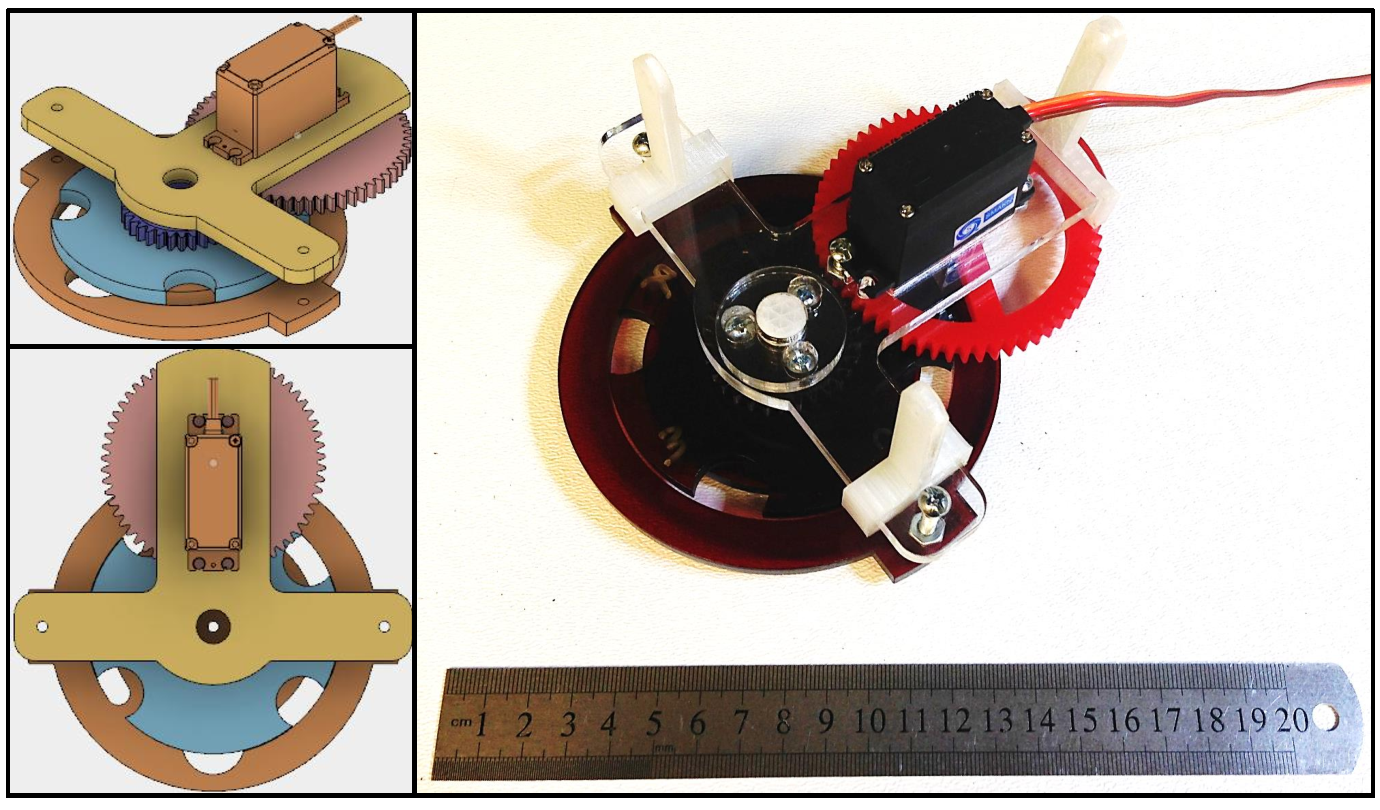
\includegraphics[width=\columnwidth]{deployment_system.pdf}}
 \caption{Deployment system for dropping smart darts from the UAV. Max capacity 4.} 
 \label{fig:TradvsAutoDrop}
\end{figure}}
\todobox{An: I want to know about the deployment unit.  }

\subsection{Experiment}


\subsubsection{Autonomous drop demonstration and accuracy}

The current drone can place the SmartDart within $\pm1$ m of the desired location.  This inaccuracy is 
1)     There are often features (rocks, water, etc.) that require this amount of error from theoretically assigned locations,
2)     some survey designs include a random placement component to improve noise cancellation,
3)     this error minimally perturbs  the data since seismic waves travel at 600 m/s in near surface, so a one-meter inaccuracy equates to $\approx$1.6 ms delay,
4)     the response of a receiver to seismic vibrations is an average over a number of meters.

The critical factor is to know exactly (within 10 cm accuracy)  the geophone location. Knowledge of this exact location allows corrections for the possible jitter in arrival times of the signal due to inaccuracy of placement.


Exp 4: Automatic drop from drone, accuracy in placement
\textbf{\begin{figure} \centering
  {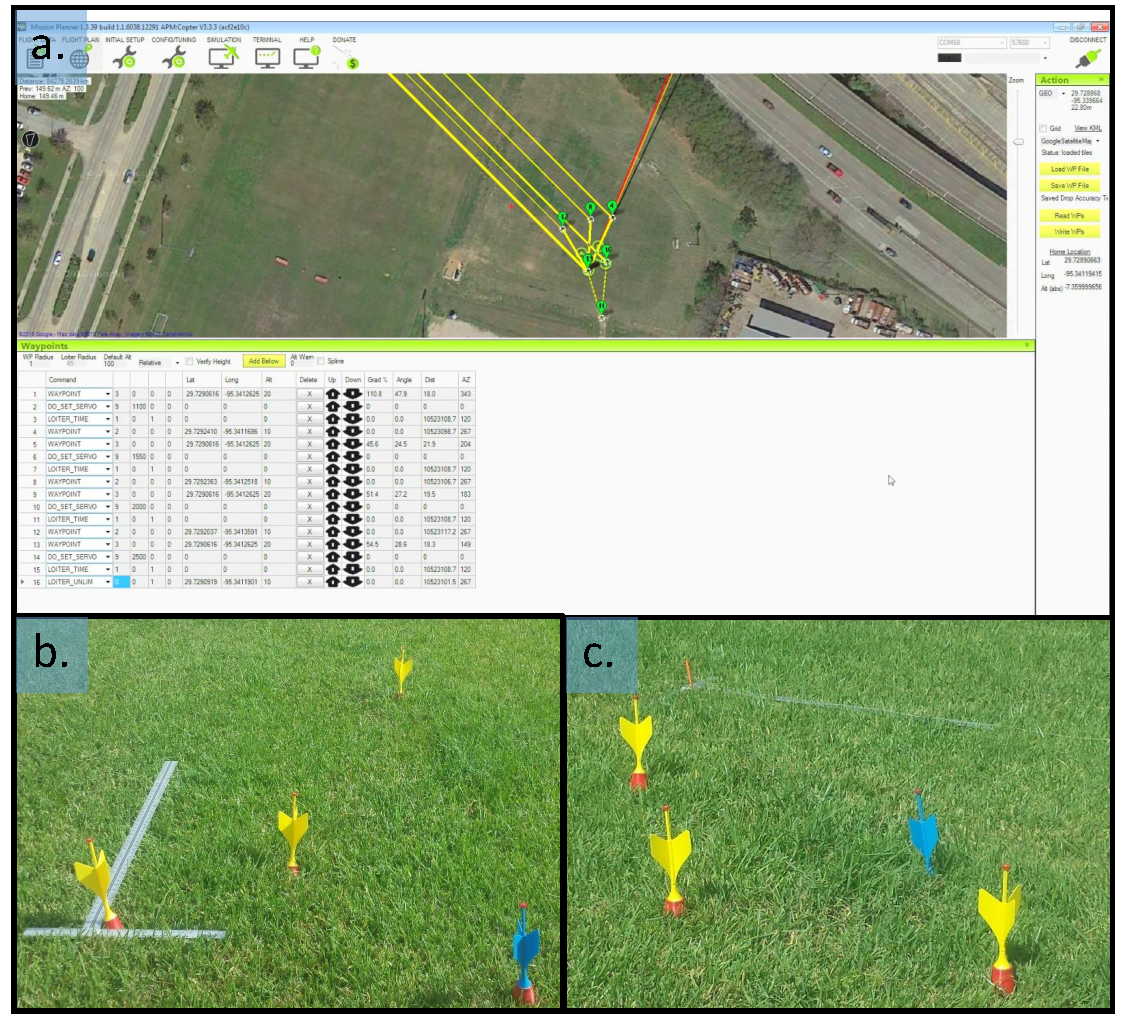
\includegraphics[width=\columnwidth]{accuracy_test_overview.pdf}}
 \caption{a.) Flight plan of accuracy test b.)First set of dart with reference axes c.)Later Dart Sets} 
 \label{fig:Accu_test_darts}
\end{figure}}
The UAS is a 177 cm wing span hexacopter, controlled by the Pixhawk flight controller running ArduPilot Mega flight software. The UAS has a 3DR GPS module using the UBlox NEO-7 chipset.

For the accuracy test, 6 sets of dart, 4 darts in each set, were dropped on the same GPS waypoint. Between each drop, the UAS travel to another GPS waypoint close by to cancel out the flight controller's stable hover as shown in Fig.~\ref{fig:Accu_test_darts}a. UAS return to launch platform to be reloaded and data is recorded after each set.

To record data, one dart was picked from the first set as the reference point (the lower left in Fig.~\ref{fig:Accu_test_darts}b), hence the first data point will be 0,0. A lager dry-wall square is placed with the origin at the dart's drop point to establish axes.

After the first set of data has been recorded, the darts are collected and reloaded on to the UAS for next set of deployment. A rod is placed in the position of the first dart to keep reference as shown in Fig.~\ref{fig:Accu_test_darts}c. The dry-wall square is kept in place, strings were tied on the ground to lengthen the reference axes. Future deployment will be compared against the reference point and axes.

\todobox{AN:  Need figure for accuracy of placement for drone drop}

\begin{figure} \centering
  {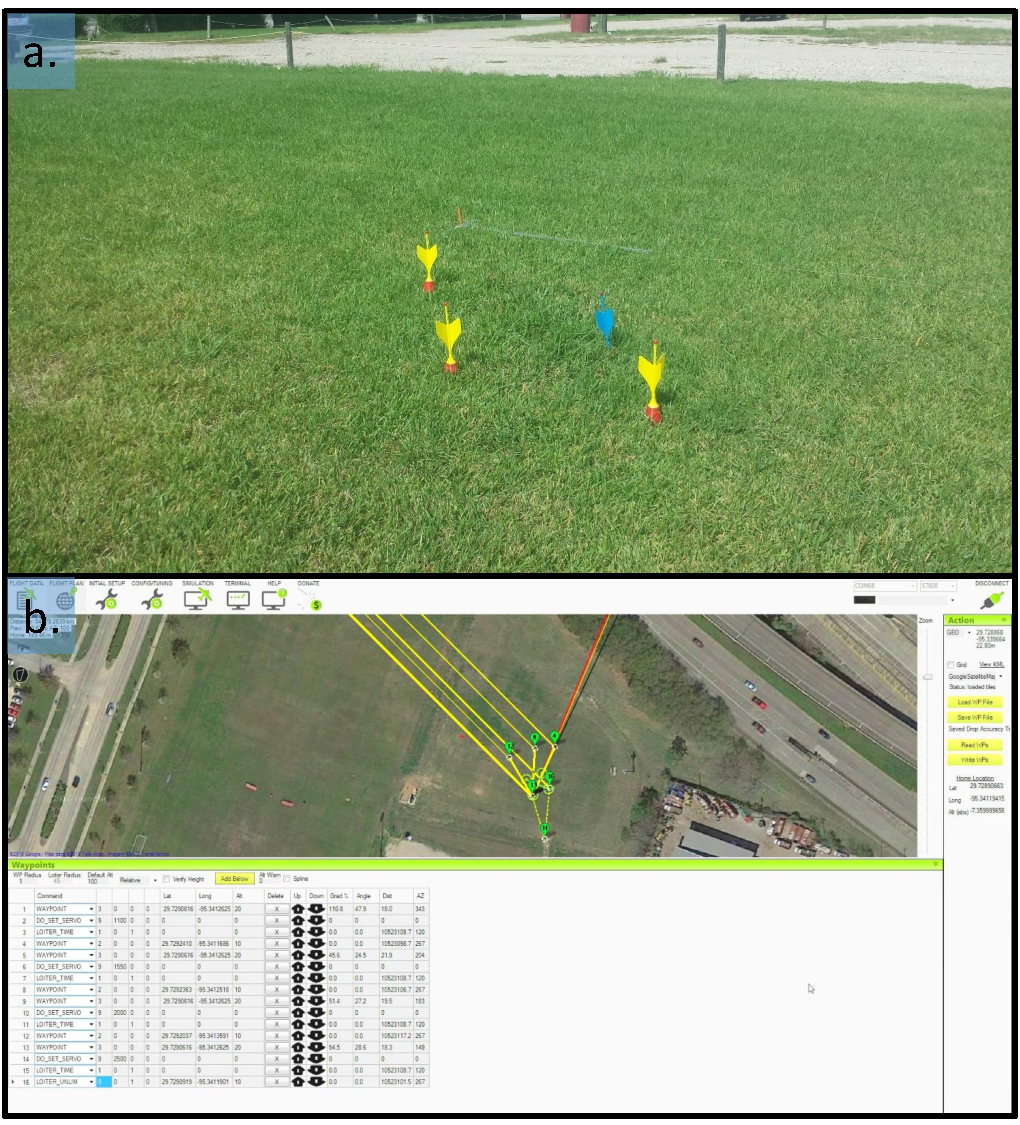
\includegraphics[width=\columnwidth]{accuracy_test_darts.pdf}}
 \caption{a.) Smart darts deployed autonomously by the deployment unit (hexacopter) b.) Screen shot of flight plan for autonomous deployment} 
 \label{fig:TradvsAutoDrop}
\end{figure}

\subsubsection{Height vs. penetration depth}
Exp 5: Height vs. penetration depth

\todobox{AN:  Need figure for accuracy of placement for drone drop}

\textbf{\begin{figure} \centering
  {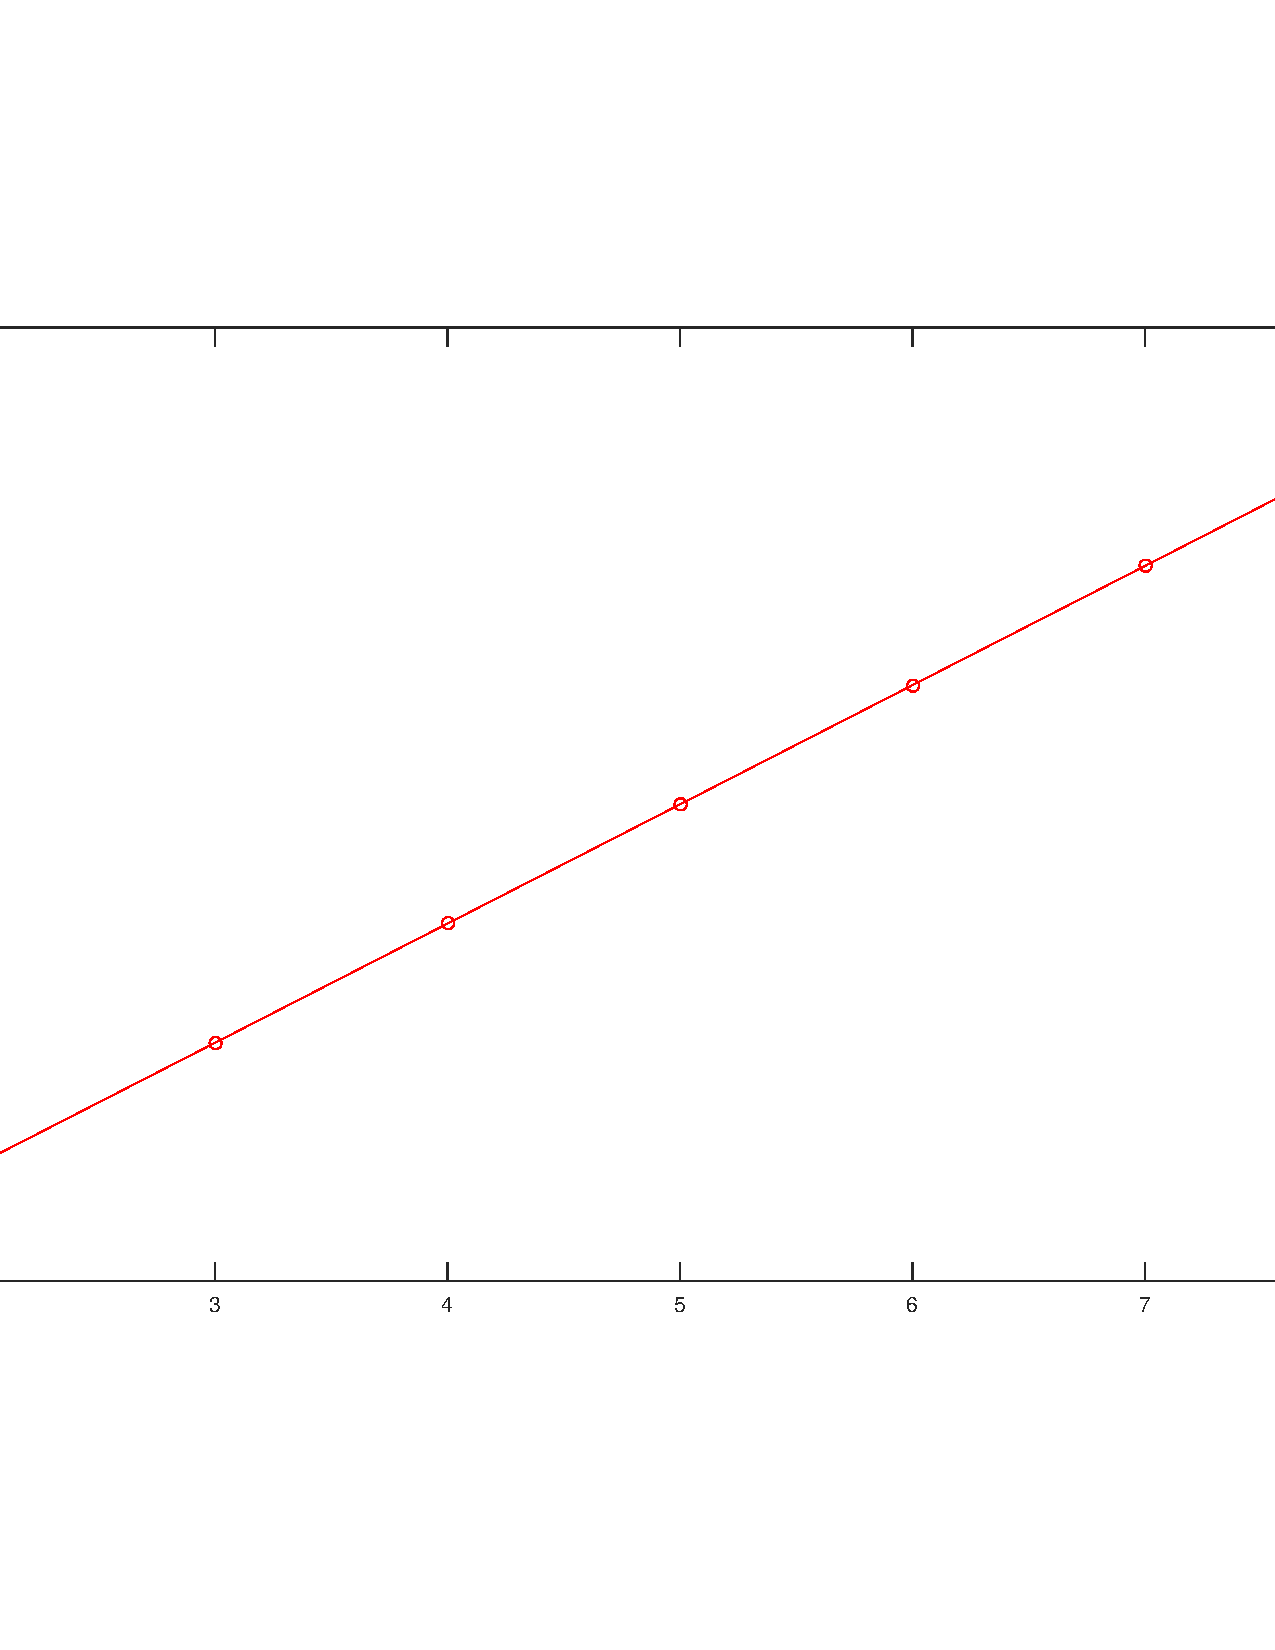
\includegraphics[width=\columnwidth]{replace_graph.pdf}}
 \caption{Plot of pneumatic cannon firing angle vs ending angle} 
 \label{fig:TradvsAutoDrop}
\end{figure}}
